\documentclass[11pt]{article}
\usepackage[paperwidth=8.5in,paperheight=11in,textwidth=5.6in,top=0.9in,bottom=0.9in]{geometry}
\usepackage[T1]{fontenc}
\usepackage{lmodern,microtype,graphicx,booktabs,xcolor,enumitem,dirtree,titlesec,float}
\usepackage[most]{tcolorbox}
\usepackage[colorlinks,urlcolor=accent,linkcolor=accent]{hyperref}
\renewcommand{\familydefault}{\sfdefault}
\definecolor{accent}{HTML}{2A78D6}
\definecolor{ink}{HTML}{0B0B0B}
\definecolor{muted}{HTML}{52514E}
\definecolor{wash}{HTML}{F3F2EE}
\setlength{\parindent}{0pt}
\setlength{\parskip}{0.6em}
\setlist{nosep,leftmargin=1.2em}
\titleformat{\section}{\Large\bfseries\color{ink}}{}{0pt}{}
\titlespacing*{\section}{0pt}{1.4em}{0.3em}
\newcommand{\f}[1]{\texttt{#1}}
\newtcolorbox{quoteit}{enhanced,breakable,colback=white,colframe=white,borderline west={3pt}{0pt}{accent},
  left=10pt,right=4pt,top=2pt,bottom=2pt,fontupper=\itshape\color{muted}}
\newtcolorbox{panel}[1][]{enhanced,colback=wash,colframe=wash,arc=4pt,left=10pt,right=10pt,#1}
\newcommand{\stat}[2]{\begin{tabular}[t]{@{}c@{}}{\huge\bfseries\color{accent}#1}\\[2pt]{\small\color{muted}#2}\end{tabular}}
\newcommand{\who}[1]{\textbf{\color{accent}#1}}

% numbers from session.py (end of session)
\newcommand{\wall}{95}\newcommand{\human}{18}\newcommand{\agent}{49}\newcommand{\usd}{7.59}

\begin{document}

{\small\color{muted}LAB NOTEBOOK \textbullet{} 2026-10-20 \textbullet{} 6 min read}\\[4pt]
{\fontsize{26}{30}\selectfont\bfseries\color{ink} An Agent Lab for Scientific\\ Software Optimization}\\[6pt]
{\large\color{muted} One scientist, one agent, one deforming bubble: a session that took a
C++/MPI solver from FP64 to ``ready to evolve'' in an afternoon, and what it cost.}

\vspace{0.8em}
\begin{panel}
\centering
\stat{\wall\,min}{session} \hfill \stat{\human\,min}{of scientist time} \hfill
\stat{\$\usd}{in tokens} \hfill \stat{1.0}{core-hour of emulation}
\end{panel}

\section{The ask}

The lab is built to lower the precision of scientific codes, safely. The code under study sits in
\f{app/} and changes with each scientist; everything around it is general. Today's app is the
Deforming Bubble, a level-set mini-app ported from Flash-X (WENO5 advection, redistance, MPI),
standing in for the DOE applications the lab is meant for. The scientist dropped it in and typed:

\begin{quoteit}
I have added my code to the app, and ready for optimization.
\end{quoteit}

The agent's first move was a polite \emph{not yet}. Optimization evolves a low-precision
\emph{seed}, and no seed existed. So it read the lab's rulebook, checked the app against its
13-point contract (all pass, natively and in Docker), and proposed the first stage instead:
\emph{raptorize}. Fourteen minutes after the ask, a plan was waiting, with every decision
filled in and its source cited. The scientist didn't have to answer a single question
to get there.

\section{Meet the lab}

\begin{figure}[H]
\begin{panel}
\small
\dirtree{%
.1 AlphaEvolve-MxP/.
.2 app/\DTcomment{\textbf{swappable}: any code meeting app.md (today: the bubble)}.
.2 dev/workflows/\DTcomment{\textbf{general}: the lab's playbook}.
.3 protocol.md\DTcomment{plan mode, run mode, checkpoints}.
.3 raptorize/ optimize/ verify/\DTcomment{one contract per stage}.
.2 experiments/2026-10-20/\DTcomment{today's question}.
.3 README.md\DTcomment{one row per run, with its commit}.
.3 1-raptorize/\DTcomment{plan.md, raptorize.patch, results/}.
.3 2-optimize/\DTcomment{plan.md, experiment.yaml, evaluator.py}.
.3 report.tex, session.py\DTcomment{this post, and its numbers}.
}
\vspace{6pt}
{\color{muted}Swap \f{app/} and the rest stays. Stages run \textbf{raptorize} $\rightarrow$ \textbf{optimize} $\rightarrow$
\textbf{verify}. Each stage is a contract in \f{dev/workflows/}; each run of it gets a folder
in \f{experiments/}. Every run starts with a \emph{plan}, then executes it, stopping at
checkpoints where only the scientist can say go.}
\end{panel}
\caption{The whole lab on one screen: the app changes, the lab doesn't.}
\end{figure}

\section{How it went}

\begin{figure}[H]
\centering
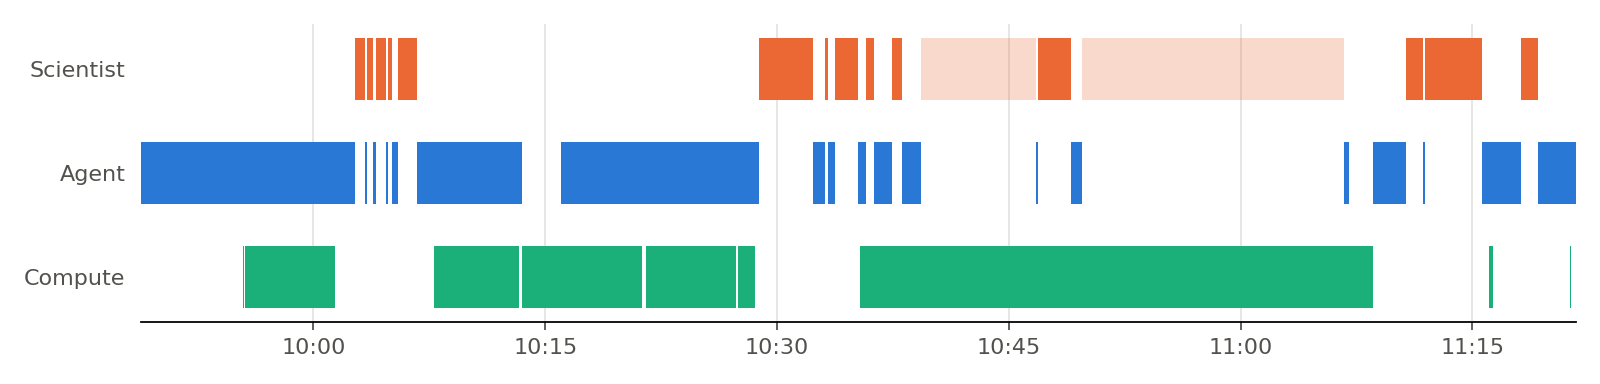
\includegraphics[width=\linewidth]{figures/timeline.png}
\caption{Who was busy when. Pale orange: the scientist was free while runs went.
The scientist's lane adds up to \human{} minutes.}
\end{figure}

Seventeen messages, 282 words from the scientist. The best moments came from the scientist
pushing back:

\who{``Why did you choose advect.cpp?''} The honest answer was ``I read the code.'' Two minutes
later there was a profile: advection 52\% of runtime, redistance 24\%. It also turned up a
wrong number in the plan, which got fixed.

\who{``Was your decision influenced by a memory?''} No. It came from the stage's default (``the
hottest loop'') and the code. A plain question, a plain answer.

\who{``Run everything inside the container.''} The agent re-ran the FP64 baseline in the
container too, so ``unchanged'' compares one compiler with itself, not two.

\who{``Can I look at some plots?''} At 100 steps the four bubble outlines were identical.
Unremarkable, so the scientist asked to \emph{run until the bubble deforms}.

\who{``The runs still working?''} Yes, but at a third of the expected speed. OpenMPI had pinned
four jobs onto two cores. One flag fixed it.

\who{``Why not 2--3 MPI ranks?''} Three doesn't divide a 128-cell grid; two does, and the field
came out bit-identical to the single-rank run in all 11 frames.

\who{``What do you mean, checkpoint 3?''} The one miss. The ``record and commit?'' question was
buried under three follow-up requests, and had to be explained again.

\section{What came out}

\begin{figure}[H]
\centering
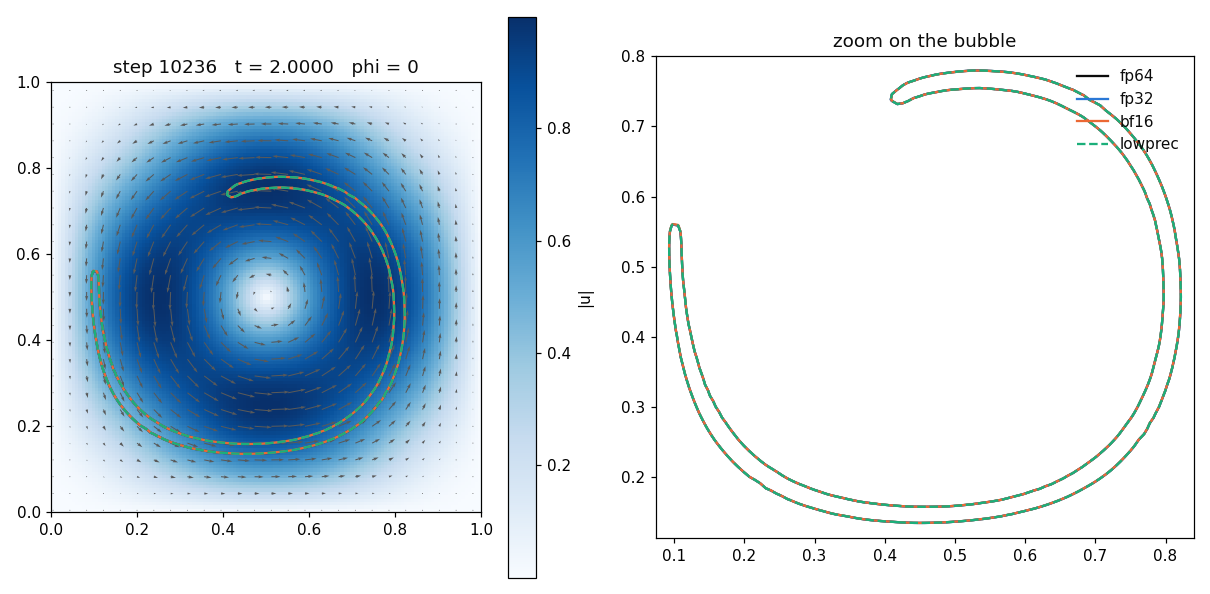
\includegraphics[width=\linewidth]{figures/full_compare_010236.png}
\caption{The bubble at $t=2$, after 10\,236 steps, in four precisions. Spot the difference:
there isn't one at this scale.}
\end{figure}

\begin{center}
\begin{tabular}{@{}lll@{}}
\toprule
mode & RMS error at $t=2$ & the short story \\
\midrule
fp32 (RAPTOR emulated) & $6.3\times10^{-7}$ & 30 min of emulation \\
float seed (native)    & $6.3\times10^{-7}$ & same answer, bit for bit, in 17 s \\
bf16 (RAPTOR emulated) & $2.6\times10^{-4}$ & 400$\times$ worse, still invisible \\
\bottomrule
\end{tabular}
\end{center}

The float seed matching emulated fp32 bit for bit is the best possible check that it's a
faithful copy. The error maps showed the error lives far from the bubble's edge, where
it barely matters. That's a hint the optimize score should look near the interface.

\textbf{Optimize, so far.} The plan, evaluator and job are written. The seed scored 9.2722 twice
(the same both times). The launch waits on Google Cloud credentials.

\section{What it cost}

\begin{center}
\begin{tabular}{@{}lrrr@{}}
\toprule
Claude Opus 5.5, 103 calls & tokens & \$/M & \$ \\
\midrule
fresh input        & 208          & 4.00  & 0.00 \\
cache writes       & 624\,107     & 5.00  & 3.12 \\
cache reads        & 13\,294\,158 & 0.20  & 2.66 \\
output             & 90\,268      & 20.00 & 1.81 \\
\midrule
\textbf{total}     &              &       & \textbf{\usd} \\
\bottomrule
\end{tabular}
\end{center}

95\% of what the model read came from the cache, at a twentieth of the price. The surprise is
that cache \emph{writes} are the biggest line. The cache lives five minutes, and this lab
waits: a half-hour run, a scientist looking at plots. Every long pause meant re-caching the
whole conversation. A one-hour cache would fit this lab better.

\section{Human time vs.\ time saved}

\begin{panel}
\begin{tabular}{@{}p{4.3in}r@{}}
\multicolumn{2}{@{}l}{\textbf{Doing it by hand} \color{muted}(our estimate, for an expert new to the lab)}\\[2pt]
read the lab rules and the app, pick and profile the kernel & 1.5 h \\
precision modes, shadow run, error columns, RAPTOR build    & 4 h \\
gate, plots, full runs (and spotting the core pinning)      & 1.5 h \\
optimize plan, evaluator, calibration                       & 1.5 h \\
write this up with figures and costs                        & 2 h \\
\midrule
\textbf{total}                                              & \textbf{$\approx$ 10 h} \\[4pt]
\textbf{With the agent:} scientist's attention              & \textbf{\human{} min} \\
\end{tabular}
\end{panel}

Roughly a 30$\times$ cut in human time, for \$\usd. Because only \f{app/} is specific, the
next DOE code reuses all of it: the contracts, the checks, and this report's script. The agent was working for \agent{} of the
\wall{} minutes. The scientist spent their time on what only a scientist can do: questioning
choices, asking for the run that matters, and widening the test.

\section{What we'd change}

\begin{itemize}
  \item \textbf{Keep open gates in view.} A pending checkpoint shouldn't scroll away.
  \item \textbf{Cache for the lab's pace:} a one-hour cache when runs take half an hour.
  \item \textbf{Score where the physics is:} an error measured near the interface for optimize.
  \item \textbf{Small papercut:} the app should create its output folder's parents.
\end{itemize}

{\small\color{muted}Numbers: \f{session.py} reads the session transcript (token usage per call,
timestamps, tool calls). Runs, plans and patches are under \f{experiments/2026-10-20/}.}

\end{document}
